\section{Bias in thresholded and weighted estimators}
\label{sec:theorems}

In this section, we derive the asymptotic biases for the thresholded estimator \eqref{demo: est_race} and weighted estimator \eqref{demo: weight} for demographic disparity. We also provide some interpretable sufficient conditions under which these two estimators overestimate or underestimate the demographic disparity.

% In this section, we explore conditions that create bias in disparity measures used to infer model fairness. Since the protected attribute is unknown, we can use relationships between the proxy estimate and the decision outcome as practical criteria for circumstances when disparity is overestimated. We look at the disparity measures using threshold cutoff from Equations \ref{demo: est_race}, \ref{cond_demo: est_race}, \ref{adj_demo: est_race} and weighting estimator method from Equations \ref{demo: weight}, \ref{cond_demo: weight}, \ref{adj_demo: weight} for estimating the unknown protected attribute.


\subsection{Weighted estimator}

\begin{theorem}\label{thm: weighted}
Let $A$ be a binary protected class with values $a$ and $b$. The bias of the weighted estimator $\hat{\delta}_{W}$ in Definition \ref{def:weighted_estimator} for demographic disparity $\delta$ in \eqref{def:demo-disparity} is
\[
\hat{\delta}_{W} - \delta = [\hat{\mu}_{W}(a) - \mu(a)] -  [\hat{\mu}_{W}(b) - \mu(b)],
\]
where as $N \to \infty$, the biases in the weighted estimators for the mean group outcomes $\hat{\mu}_{W}(u)$, for $u\in\{a,b\}$, converge almost surely to
\begin{equation}
\hat{\mu}_{W}(u) - \mu(u) \xrightarrow{\textrm{a.s.}} -\frac{\expect [\cov (\ind(A = u), Y \mid Z)]}{\pr (A = u)}.\label{formula: weight-bias1}
\end{equation}

\end{theorem}

We omit the $a.s.$ (almost sure) notation later for brevity.

\begin{corollary}
\label{corr:weighted-unbiased}
If $Y$ is independent of $A$ conditionally on $Z$, then the weighted estimator for demographic disparity, $\hat{\delta}_{W}$, is asymptotically unbiased.
\end{corollary}

If $Y$ is independent of $A$ conditionally on $Z$, then the advantaged group and disadvantaged group with the same $Z$ values are equally treated in terms of the average outcome.
Nevertheless, this does not contradict the existence of overall disparity against the disadvantaged group in terms of the unconditioned average outcome, as an example of Simpson's paradox \cite{Simpson1951}.
The conditional independence assumption required by Corollary \ref{corr:weighted-unbiased}
is trivially satisfied if $Y$ is the output of some function $f(X)$, and $Z$ includes the input features $X$, since $Y$ is now determined entirely by $Z$.
Such a situation arises naturally when $Y$ is the output of machine learning algorithms. In the Appendix \ref{section: unbiased_weighted}, we show a semi-synthetic example based on the mortgage dataset where the weighted estimator is asymptotically unbiased when the proxy model is well constructed so that the conditional independence assumption is satisfied.

However, this conditional independence assumption may not hold in practice and the weighted estimator may be biased. Consider the example of loan application with race proxy based on geolocation. If within most locations, the affirmative action described in Example \ref{ex:affirmative_action} is present, i.e., the disadvantaged group is more likely to get a loan than their neighbors from the advantaged group, then $Y$ covaries negatively with $\ind(A = a)$ and positively with $\ind(A = b)$ conditionally on $Z = z$, for most values of $z \in \mathcal{Z}$, which implies that the weighted estimator overestimates the demographic disparity. On the contrary, if within most locations, the advantaged group is more likely to get loan than their neighbors belonging to the disadvantaged group, then $Y$ covaries in the exact opposite way, implying that the weighted estimator underestimates the demographic disparity. Overall, the estimation bias of the weighted estimator depends on the intra-geolocation variation of the loan application outcome.

%The intuition we build from these examples will be useful to understand the more complex results on a real mortgage data set in Section \ref{sec:mortgage}.

% \begin{theorem}
% Consider $x \in \mathcal{X}$. When $h \to 0$, $Nh \to \infty$, and $A \perp X \mid Z$, the asymptotic bias of the kernel weighted estimator $\hat{\delta}^{(w)}(x)$ in eq. \eqref{cond_demo: weight} for conditional demographic disparity $\delta(x)$ in eq. \eqref{def:cond-demo-disparity} is
% \begin{align*}
%     \plim \hat{\delta}^{(w)}(x) - \delta(x) &= \frac{\expect [\cov (\ind(A = b), Y \mid Z, X = x) \mid X = x]}{\pr (A = b \mid X = x)} \\
%     &-  \frac{\expect [\cov (\ind(A = a), Y \mid Z, X = x) \mid X = x]}{\pr (A = a\mid X = x)}
% \end{align*}
% \end{theorem}


% \begin{corollary}
% When $h \to 0$, $Nh \to \infty$, $N' \to \infty$, and $A \perp X \mid Z$, the asymptotic bias of the kernel weighted estimator $\hat{\Delta}^{(w)}$ in eq. \eqref{adj_demo: weight} for the adjusted demographic disparity $\Delta$ in eq. \eqref{def:adj-demo-disparity} is
% \begin{align*}
% \plim \hat{\Delta}^{(w)} - \Delta &= \expect_X \bigg\{\frac{\expect [\cov (\ind(A = b), Y \mid Z, X) \mid X]}{\pr (A = b \mid X)} \\
% &\quad \quad \quad - \frac{\expect [\cov (\ind(A = a), Y \mid Z, X) \mid X]}{\pr (A = a\mid X)}\bigg\}.
% \end{align*}
% \end{corollary}


% \paragraph{Demographic disparity: the weighting estimator is asymptotically unbiased for if $Y \perp A \mid Z$.}
% \begin{itemize}
%   \item However, this does not mean that $Y \perp A$ because $Y$ may be dependent with $Z$. Actually it is possible that $Y \perp A \mid Z$ but $Y$ is dependent with $A$ when $Y$ is dependent with $Z$. (Note that we had some misunderstanding regarding this before when we said that the weighting estimator is accurate only if there is no disparity. This is not true! Look one example below.)
%   \item This means that if $Z$ blocks all dependence between $Y$ and $A$, then using weighting estimator is accurate. For example, if $Y$ is the output from a machine learning algorithm, and $Z$ contains all input features used in the algorithm that are correlated with $A$, then this conditional independence assumption is trivially satisfied since $Y$ is deterministic conditionally on the all input features. However, this may not be practically useful since it is hard to get dataset containing true race label and the relevant features so that we can train the probabilistic proxy. Nevetheless, it is still meaningful for practitioners to consider including input features that are available and strongly correlated with $A$ in $Z$;
%   \item This condition captures the variation of received decision outcome within all leves of the predictor for estimating the unknown protected attribute. This condition is neither necessary nor sufficient for (c)(d) in conditions (*) described in Theorem \ref{thm: demographic-est-race} (again consider Simpson paradox).
% \end{itemize}

% \paragraph{Demographic disparity: consider the example where the protected attribute is race, geolocation is used to estimate race, and the decision outcome is the credit decision.}
% \begin{itemize}
%   \item Within the same geolocation, if people in the historically disadvantaged group $b$ are more likely to be accepted while the historically advantaged group $a$ are more likely to be rejected ($\cov (\ind(A = b), Y \mid Z) > 0$ but $\cov (\ind(A = a), Y \mid Z) < 0$), then the weighting estimator overestimates the demographic disparity.
%   \item Within the same geolocation, if group $b$ are more likely to be rejected while group $a$ are more likely to be accepted ($\cov (\ind(A = b), Y \mid Z) < 0$ but $\cov (\ind(A = a), Y \mid Z) > 0$), then the weighting estimator underestimates the demographic disparity.
%   \item Let's describe one example where $Y \perp A \mid Z$ doesn't imply $Y \perp A$ (essentially Simpson Paradox). Suppose we have two locations: one location with above-average socioeconomic status $z_1$ and one location with below average socioeconomic status $z_2$, both of which have population of 100 people. In location $z_2$, there are 90 people in group $b$ and 10 people in group $a$, all of whom have credit acceptance rate $20\%$. In location $z_1$, there are 10 people in group $b$ and 90 people in group $a$, all of whom have acceptance rate $80\%$. Therefore, in each location, people in groups $a$ and $b$ are equally likely to get credit ($Y \perp A \mid Z$). However, the overall acceptance rate for the advantage group $a$ is $74\%$ while the overall acceptance rate for the disadvantaged group $b$ is $26\%$ ($Y$ is dependent with $A$).
% \end{itemize}

\subsection{Thresholded estimator}

Before stating the asymptotic bias for the estimator \eqref{demo: est_race}, we define the following terms for $u \in \{a, b\}$:
\begin{align*}
    \Delta_1(u) = &\; \expect [Y \mid \pr(A = u \mid Z) > q, A = u^c]\\
    & - \expect [Y \mid \pr(A = u \mid Z) > q, A = u], \\
    \Delta_2(u) = &\; \expect [Y \mid \pr(A = u\mid Z) \le q, A = u] \\
    & - \expect [Y \mid \pr(A = u\mid Z) > q, A = u],
\end{align*}
where $q$ is the threshold used for estimating race, and $u^c$ is the class opposite to $u$, i.e., $u^c = b$ if $u = a$ and $u^c = a$ if $u = b$. $\Delta_1(u)$ measures the outcome mean discrepancy for two different protected groups \textit{within} the same proxy probability range, and $\Delta_2(u)$ measures the outcome mean discrepancy \textit{across} different proxy probability ranges for the same protected group. Consider the example of loan application with race proxy based on geolocation. In this example, $\Delta_1(u)$ measures the loan approval disparity between two race groups who live in locations that are primarily occupied by one of these two races (in terms of the threshold $q$). In contrast $\Delta_2(u)$ measures the loan approval rate disparity between people belonging to a race who live in locations that are primarily occupied by this race group and people belonging to this race who live in locations that are less occupied by this race. Therefore, $\Delta_1(u)$ roughly characterizes the \textit{intra-geolocation} variation of loan outcome and $\Delta_2(u)$ roughly characterizes the \textit{inter-geolocation} variation of loan outcome.

\begin{theorem} \label{thm: demographic-est-race-bias}
Let $A$ be a binary protected class with values $a$ and $b$. 
The bias for the thresholded estimator $\hat{\delta}_q$ in Definition \ref{def:thresholded_estimator} is:
\[
\hat{\delta}_{q} - \delta = [\hat{\mu}_{q}(a) - \mu(a)] -  [\hat{\mu}_{q}(b) - \mu(b)],
\]
and as ${N \to \infty}$, for $u \in \{a, b\}$ and $u^c \in \{a, b\}$ as the class opposite to $u$, 
\begin{align*}
    \hat{\mu}_{q}(u) - \mu(u) \to &\;\Delta_1(u)C_1(u) - \Delta_2(u)C_2(u) \\
    &+ (\Delta_1(u) - \Delta_2(u))C_3(u),
\end{align*}
where
\begin{align*}
    C_1(u) & = \pr(\hat{A} = u \mid A = u)\pr(A = u^c \mid \hat{A} = u), \\
    C_2(u) & = \pr(A = u \mid \hat{A} = u)\pr(\hat{A} \ne u \mid A = u)\textrm{, and}\\
    C_3(u) & = \pr(\hat{A} \ne u \mid A = u)\pr(A = u^c \mid \hat{A} = u).
\end{align*}
Here $\hat{A} \ne u$ means that $\hat{A} = u^c$ or $\hat{A} = \text{NA}$.
\end{theorem}
%
The generalization to multiclass $A$ is straightforward and in Appendix \ref{section:theory_bias} we show that the bias formula in Theorem \ref{thm: demographic-est-race-bias} for binary protected class capture the main effects of the bias for multiclass $A$.

Theorem \ref{thm: demographic-est-race-bias} shows that the occurrence of overestimation or underestimation depends on complex interplay of the $\Delta$ terms. In the following corollary, we provide the simplest set of sufficient conditions for the overestimation and underestimation to demonstrate the main intuition.

\begin{corollary} \label{corollary: demographic-est-race}
Suppose
\begin{subequations}
\begin{align}
  \Delta_1(a) &\ge 0,\tag{5i}\label{eq:condition1} \\
  -\Delta_1(b) &\ge 0,\tag{5ii}\label{eq:condition2} \\
 -\Delta_2(a) &\ge 0,\tag{5iii}\textrm{ and} \label{eq:condition3}\\
  \Delta_2(b) &\ge 0,\tag{5iv}\label{eq:condition4}
\end{align}
\end{subequations}
and at least one inequality holds strictly.
Then in the limit $N\!\rightarrow\!\infty$,
$\hat{\mu}_q(a) > \mu(a)$, $\hat{\mu}_q(b) < \mu(b)$, and $\hat{\delta}_q > \delta$, i.e. the thresholded estimator overestimates the demographic disparity.

Conversely, let \begin{enumerate*}[label=(\roman*\ensuremath{^\prime})]
\item $\Delta_1(a)\!\le\!0$,
\item $\,-\Delta_1(b)\!\le\!0$,
\item $\,-\Delta_2(a)\!\le\!0$, and
\item $\Delta_2(b)\!\le\!0$,
\end{enumerate*}
and at least one inequality holds strictly.
Then in the limit $N\rightarrow\infty$,
$\hat{\mu}_q(a) < \mu(a)$, $\hat{\mu}_q(b) > \mu(b)$, and $\hat{\delta}_q < \delta$, i.e. the thresholded estimator underestimates the demographic disparity.
\end{corollary}

The conditions \eqref{eq:condition1}---\eqref{eq:condition4} are demonstrated in Figure \ref{figure: theorem}.
% The following proposition shows that conditions  \eqref{eq:condition1}---\eqref{eq:condition2} are closely related to the bias terms in Theorem \ref{thm: weighted} for the weighted estimator. This leads us directly to the following theorem:

% \begin{theorem}\label{prop: relation-weighted-thresholding}
% Let the estimated labels $\hat{A}$ be defined as in Definition \ref{def:thresholding_rule}, and
% assume that the $\hat{A}$s are more likely than not to match the true labels $A$, namely
% $\pr (\hat{A} = a \mid A = a) \ge \pr (\hat{A} = a \mid A = b)$, and
% $\pr (\hat{A} = b \mid A = b) \ge \pr (\hat{A} = b \mid A = a)$.
% %
% Then
% \begin{enumerate}[label=(\alph*)]
% \item[(a)] if $\cov (\ind(A = a), Y \mid Z = z) < 0$ and $\cov (\ind(A = b), Y \mid Z = z) > 0$ for any $z$, then $\Delta_1(a) > 0$, $\Delta_1(b) > 0$, and $\hat{\delta}_W > \delta$, i.e. the weighted estimator overestimates the demographic disparity. Conversely,
% \item[(a')] if $\cov (\ind(A = a), Y \mid Z = z) > 0$ and $\cov (\ind(A = b), Y \mid Z = z) < 0$ for any $z$, then $\Delta_1(a) < 0$, $\Delta_1(b) < 0$, and $\hat{\delta}_W < \delta$, i.e. the weighted estimator underestimates the demographic disparity.
% \end{enumerate}
% \end{theorem}

% Theorem \ref{prop: relation-weighted-thresholding} assumes that the probabilistic proxy is reasonably predictive of the true labels $A$, and furthermore describe sufficient conditions under which $\Delta_1(a)$ and $\Delta_1(b)$ never cancel, resulting in a consistent over- or underestimate.
% In the example of loan application with race proxy based on geolocation, conditions  \eqref{eq:condition1}--- \eqref{eq:condition2} also capture the \textit{intra-geolocation} variation as the covariance terms in Theorem \ref{thm: weighted}.

Conditions \eqref{eq:condition1}---\eqref{eq:condition2} exactly formalize the intuition captured by Example \ref{ex:affirmative_action}.
In our loan application example, using a geolocation-based race proxy, these two conditions capture the intra-geolocati\-on outcome variation:
on average higher proportion of disadvantaged group $b$ receive the favorable outcome than the advantaged group $a$ among all the geolocations that are primarily occupied by one race (in terms of the threshold $q$).

The conditions \eqref{eq:condition3}---\eqref{eq:condition4} exactly formalize the intuition captured by Example \ref{ex:income}.
They characterize the dependence between the decision outcome and the proxy probability conditionally on the protected attribute.
Specifically, condition \eqref{eq:condition3} holds when the decision outcome is positively correlated with the probability of belonging to the advantaged group, while condition \eqref{eq:condition4} holds when the decision outcome is negatively correlated with the probability of belonging to the disadvantaged group conditionally on the true protected attribute.
In the example of loan application with race proxy based on geolocation, geolocation is correlated with both race ratio and socioeconomic status (e.g., income, FICO score, etc.): locations that are primarily occupied by the advantaged racial groups tend to be associated with relatively higher socioeconomic status while locations that are primarily occupied by the disadvantaged racial groups tend to be associated with relatively lower socioeconomic status.
As a result, people who live in locations dominant by the advantaged racial group are assigned with high probability of belonging to the advantaged group, and they are more likely to get approved in loan application because of relatively higher socioeconomic status.
% In this way, the loan approval is positively correlated with the probability of belonging the advantaged group.
% In contrast, people who live in locations that are primarily occupied by disadvantaged racial groups are assigned with high probability of belonging to disadvantaged groups, and they are less likely to get approved in loan application because of their relatively lower socioeconomic status.
% In this way, the loan approval is negatively correlated with the probability of belonging to disadvantaged groups.
Conversely, the loan approval is negatively correlated with the probability of belonging to disadvantaged groups.
% Although this example may oversimplify the reality, it clearly demonstrates that conditions \eqref{eq:condition3}---\eqref{eq:condition4} are likely to hold when the predictors $Z$ for the unknown protected attribute are also strongly correlated with the decision outcome, e.g., the geolocation is correlated with the loan approval because of the socioeconomic status disparity correlated with the geolocation.
This example demonstrates that \eqref{eq:condition3}---\eqref{eq:condition4} are likely to hold when the predictors $Z$ are also strongly correlated with the decision outcome, e.g., the geolocation is correlated with the loan approval because of the socioeconomic status disparities across different geolocations.

\begin{figure}
\centering
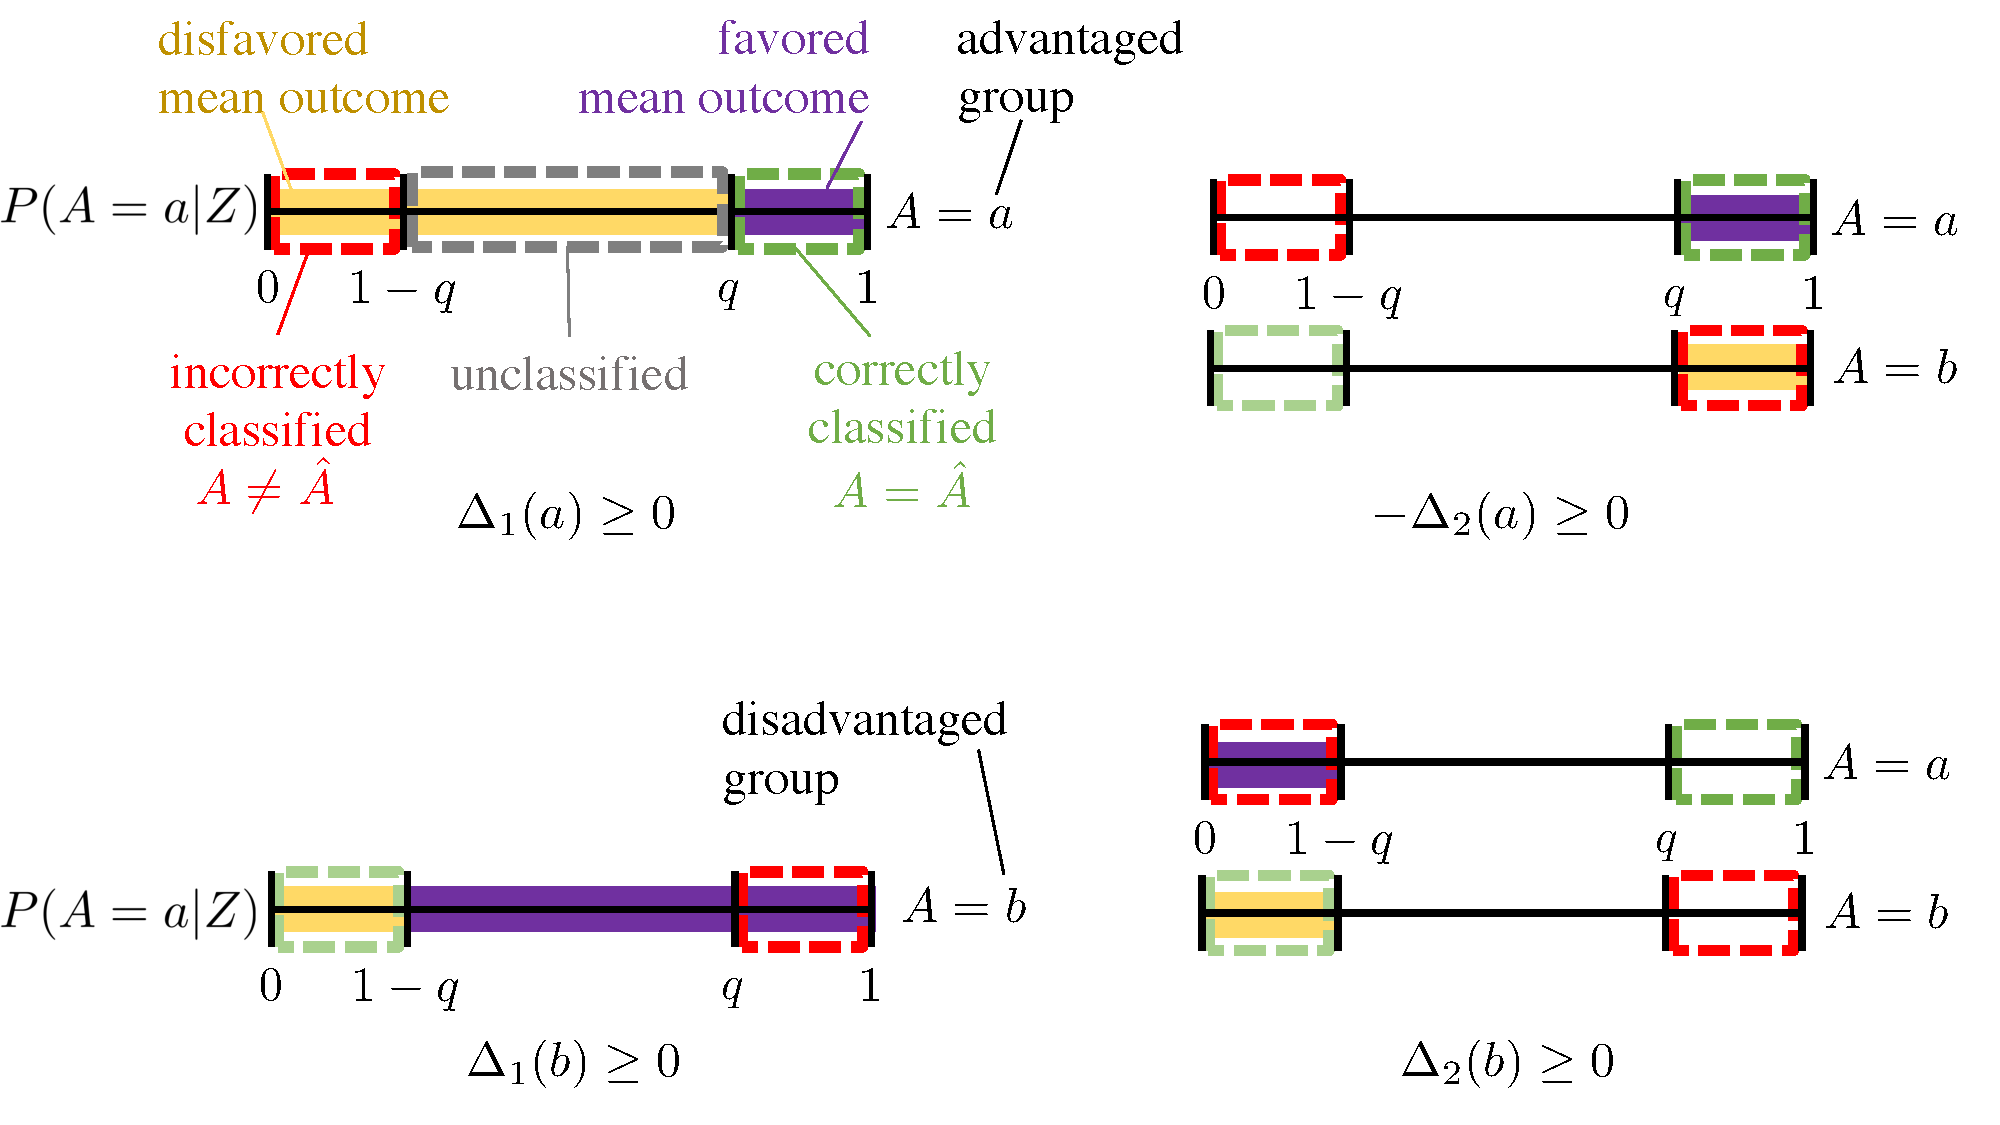
\includegraphics[width=\linewidth]{theorem_condition.pdf}
  \caption{Illustration of conditions \eqref{eq:condition1}---\eqref{eq:condition4} in Corollary \ref{corollary: demographic-est-race}, illustrating the complex interplay between membership in a protected class $A$ and outcome $Y$ that give rise to overestimated demographic disparity using the thresholded estimator of Definition \ref{def:thresholded_estimator}.
  The horizontal axes show $\pr({A}=a|Z)$, the probability that a probabilistic proxy model predicts membership in the advantaged group $a$.
  Dashed boxes represent correct ($\hat{A}=A$, green) and incorrect classifications ($\hat{A}\ne A$, red), from the thresholded estimated membership rule of Definition \ref{def:thresholding_rule}, with the interval $(1-q,q)$ always unclassified.
  Solid bars represent favored (purple) and disfavored mean outcomes (yellow).
} \label{figure: theorem}
\end{figure}

The following corollary shows that \eqref{eq:condition1}---\eqref{eq:condition4} have effects with different magnitudes on the overestimation bias:
\begin{corollary} \label{corollary: C-functions}
Let $A$ be a binary protected class with values $a$ and $b$. For $u \in \{a, b\}$ and $u^c$ as the class opposite to $u$, the quantities $C_1(u), C_2(u), C_3(u)$ in Theorem \ref{thm: demographic-est-race-bias} are related in the following way:
\begin{enumerate}[label=(\roman*)]
    \item $C_2(u) > C_3(u)$ if and only if
        \begin{equation}\label{c_value_23}
        \pr (A = u \mid \hat{A} = u) > \pr (A = u^c \mid \hat{A} = u).
        \end{equation}
    % \item If $\pr (\hat{A} = u \mid A = u) > \pr (\hat{A} \ne u \mid A = u)$, then $C_1(u) > C_3(u)$;
    \item $C_2(u) > C_1(u)$ if and only if
        \begin{equation}\label{c_value_21}
        \pr (A = u) > \pr (\hat{A} = u)
        \end{equation}
\end{enumerate}
Thus if the conditions \eqref{c_value_23} and \eqref{c_value_21} both hold, then $C_2(u) > C_1(u)$ and  $C_2(u) >C_3(u)$.
\end{corollary}

Condition \eqref{c_value_23} holds as long as the proxy model is reasonably predictive of the true protected class. Condition \eqref{c_value_21} usually holds for the thresholded estimated membership (Definition \ref{def:thresholding_rule}) when a high threshold $q$ is used: a fairly high fraction of observations are unclassified under the thresholded estimation rule with high threshold $q$, so the fraction of observations  classified into one protected class is usually lower than the fraction of observations actually belonging to that  protected class.
Therefore, when a high threshold $q$ is used, usually conditions \eqref{eq:condition3}---\eqref{eq:condition4} contribute more to the overestimation bias than \eqref{eq:condition1}---\eqref{eq:condition2}.
As a result, even if \eqref{eq:condition1}---\eqref{eq:condition2} are violated, as long as \eqref{eq:condition3}---\eqref{eq:condition4} hold, the thresholded estimator is still very likely to overestimate demographic disparity.
In contrast, when a low threshold is used, the difference between $\pr (A = u) > \pr (\hat{A} = u)$ is usually smaller, and thus $C_2(u) - C_1(u)$ is also smaller.
In this case, \eqref{eq:condition1}---\eqref{eq:condition2} and \eqref{eq:condition3}---\eqref{eq:condition4} may have comparable contribution to the estimation bias.
In Section 4.2, we will verify these facts by using different thresholds on the mortgage dataset.


% \subsubsection{Implications and interpretation}



% \begin{itemize}
%   \item Condition (a)(b) reflects the dependence between the decision outcome and the probabilistic proxy conditionally on the protected attribute, and we call the associated bias \textbf{type I bias}; this condition captures our main intuition regarding the bias of using probabilistic proxy, i.e., the probabilistic proxy might be correlated with the outcome in a systematic way. Take the geolocation and race proxy as an example. These two conditions mean that locations that are occupied by higher proportion of people in racial group $a$ are more likely to receive the favorable decision outcome while locations that are occupied by higher proportion of people in racial group $b$ are less likely to receive the favorable decision outcome. These two conditions characterize the \textbf{variation of recieved decision outcome \textit{across} different levels of the predictors for unknown protected attribute}, e.g., the decision oucome variation across different locations when using geolocation as the predictor for race.
%   \item Condition (c)(d) reflects the dependence between the decision outcome and the protected attribute conditionally on the range of the probabilistic proxy, and we call the associated bias \textbf{type II bias}. In the context of geolocation and race proxy, this condition means that people in group $b$ who live in locations that are primarily occupied by either people in $a$ or $b$ have no less chance of receiving the favorable decision outcome than their neighbors in group $a$, which means that people in $b$ are not disadvantaged group when conditioning on the locations that are predominantly either race. These two conditions characterize the \textbf{variation of received decision outcome \textit{within} levels of the predictor that are associated with high probability of a certain protected group}.
%   \item It is not immediately clear how plausible this condition (c)(d) are and we can validate this in the real mortgage dataset. It is likely that these two conditions only hold approximately (subject to slight violation) and the type I bias is the main source of bias. If all conditions are verified in real dataset, then we don't need to present the sufficient and necessary condition in the paper body since it is too complicated and messy.
% \end{itemize}


% \subsection{Conditional disparity overestimation from threshold cutoff proxy}

% \begin{theorem} \label{thm: cond-demo-est-race-overestimate}
% Consider the setting in Theorem \ref{thm: demographic-est-race}, and the legitimate factors $X$ that are used to adjust for observed disparity as defined in section 2. Under the following four conditions (**):
% \begin{enumerate}[label=(\alph*)]
%   \item $\expect [Y \mid \pr(A = a\mid Z) > t, A = a, X = x] - \expect [Y \mid \pr(A = a\mid Z) \le t, A = a, X = x] > 0$;
%   \item $\expect [Y \mid \pr(A = b \mid Z) \le t, A = b, X = x] - \expect [Y \mid \pr(A = b \mid Z) > t, A = b, X = x] > 0$;
%   \item $\expect [Y \mid \pr(A = a\mid Z) > t, A = b, X = x] - \expect [Y \mid \pr(A = a\mid Z) > t, A = a, X = x] \ge 0$;
%   \item $\expect [Y \mid \pr(A = b \mid Z) > t, A = b, X = x] -  \expect [Y \mid \pr(A = b \mid Z) > t, A = a, X = x] \ge 0$,
% \end{enumerate}
% where $x \in \mathcal{X}$ is a certain point in the value space of $X$.
% The estimator $\hat{\delta}(x)$ in eq. \eqref{cond_demo: est_race} based on the estimated protected attribute overestimates $\expect (Y \mid {A} = a, X = x)$ but underestimates $\expect (Y \mid {A} = b, X = x)$ asymptotically ($Nh \to \infty$ and $h \to 0$).
% As a result, $\hat{\delta}(x)$ overestimates the conditional demographic disparity $\delta(x)$ in eq. \eqref{def:cond-demo-disparity} asymptotically, i.e., $\plim \hat{\delta}(x) > \delta(x)$.
% On the contrary, when all inequalities in conditions (**) hold with the opposite direction, $\hat{\delta}(x)$ underestimates the conditional demographic disparity $\delta(x)$ asymptotically, i.e., $\plim \hat{\delta}(x) < \delta(x)$.
% \end{theorem}

% \begin{corollary}
% If conditions (**) hold for all $x \in \mathcal{X}$, then the estimator $\hat{\Delta}$ in eq. \eqref{adj_demo: est_race} based on estimated protected attribute overestimates the adjusted demographic disparity $\Delta$ in eq. \eqref{def:adj-demo-disparity} asymptotically ($Nh \to \infty$, $h \to 0$ and $N' \to \infty$), i.e., $\plim \hat{\Delta} > \Delta$. On the contrary, if conditions (**) hold with the opposite directions for all $x \in \mathcal{X}$, then $\hat{\Delta}$ underestimates the adjusted demographic disparity $\Delta$ asymptotically, i.e., $\plim \hat{\Delta} < \Delta$.
% \end{corollary}

% \subsubsection{Implications and interpretation}

% \paragraph{Conditioning on factors $X$ makes both type I bias and type II bias smaller.}
% \begin{itemize}
%   \item For example, if we believe that it is income that is correlated with both the probabilistic proxy and the outcome and thus causes type I bias, then we can condition on income and the type I bias will disappear. If in reality, the type II bias is practically negaligiable and conditioning on $X$ almost eliminates type I bias, then using estimated race would estimate disparity accurately. This means that demographic disparity (without adjusting for any factors) is the most susceptible to the estimation bias when using estimated race; unfortunately, demographic disparity was actually used by CFPB.
%   \item However, this doesn't mean that we should condition on arbitrary factors. Whether we should condition on a cetain factor depends whether this factor is a legitimate factor for justifying observed disparity. Consider a ridiculous example where credit decision depends on the color of car the applicant owns and somehow the probabilistic proxy is also correlated with the color of car. In this case, we shouldn't condition on color of car because it is not legitimate business factor. Whenever there exists factors that are correlated with both the probabilistic proxy and the outcome while they should not be adjusted for, disparate impact evaluation based on the estimated race is susceptible to the type I bias. This reflects the intrinsic limitation of using proxy in place of true protected attribute.
% \end{itemize}




% \paragraph{Conditional demographic disparity: the kernel weighted estimator is asymptotically unbiased if $Y \perp A \mid Z, X = x$.}
% \begin{itemize}
%   \item On the one hand, the $Y \perp A \mid Z, X = x$ is more likely to hold after we condition on factors $X$; on the other hand, we need another assumption $A \perp X \mid Z$, which is satisfied if $X \subset Z$, i.e., we also use $X$ when construct the probabilistic proxy. However, in practice it may be hard to find dataset that contains both ground truth and factors $X$ so that we can the probability of the membership to a protected group conditionally on $X$. This once again reflects the intrinsic limitation of using proxy in place of true protected attribute.
% \end{itemize}

% [\textbf{To do: extend the result to the conditional case}]. It's much harder to analyze the following bias term because that the denominators are different.
% \[
% \frac{\expect [\pr (A = a\mid Z)Y \mid X = x]}{\expect [\pr (A = a\mid Z) \mid X = x]} - \frac{\expect [\ind (A = a)Y \mid X = x]}{\expect [\ind (A = a) \mid X = x]}
% \]


% It seems that here the problem is quite different because we are analyzing the case where probability proxy is used as the regressor in linear regression. We may use more general nonlinear regression instead and then extrapolate the regression function to $P(A = a\mid Z) = 1$ and $P(A = b \mid Z) = 1$. In this case, we may analyze $\expect (Y \mid \pr(A = a\mid Z) = 1) - \expect (Y \mid A = a)$ and then the result will resemble the result of using estimated race, which will be totally different from the current result.
